\documentclass[11pt]{beamer}
\usetheme{Boadilla}
\usepackage{hyperref}
\usepackage[utf8]{inputenc}
\usepackage[czech]{babel}
\usepackage[T1]{fontenc}
\usepackage{amsmath}
\usepackage{amsfonts}
\usepackage{amssymb}
\usepackage{graphicx}
\usepackage{listings}
\author{Jan Tušil}
\title{An Executable Formal Semantics of C++}
%\setbeamercovered{transparent} 
%\setbeamertemplate{navigation symbols}{} 
%\logo{} 
\institute{FI MU} 
\date{1.2.2017} 
%\subject{} 


\lstset {
	basicstyle=\ttfamily
}

\newcommand{\backupbegin}{
   \newcounter{finalframe}
   \setcounter{finalframe}{\value{framenumber}}
}
\newcommand{\backupend}{
   \setcounter{framenumber}{\value{finalframe}}
}


\begin{document}


% Osnova:
% Kdo jsem - Muj obor (PdS), 
% Kontext
% Cile prace
% Co se podarilo
% Dalsi kroky
% Co chci zminit:
% - kdo me vedl, s kym jsem praci konzultoval, UIUC, RV


% Koho mam v komisi? Pelanek, Strejcek, Hlineny. Vsichni trochu do tech formalnich
% metod vidi. Strejda praci cetl, tedy musim se ji snazit prodat hlavne Pelankovi a Hlinenemu.
% Nesmim se poustet do spekulaci.
% K tomu, ze jsem nasel chyby v Gcc a Clang, a nejakou nejednoznacnost ve standardu:
% to neni tim, jaky jsem borec. To se proste stava, kdyz nekdo neco formalizuje. Kdyz lidi
% pracovali na semantice JavaScriptu, take nasli chyby v interpreterech. A ted behem praci
% na formalizaci Etherea.

% K cemu je ta semantika dobra? Jak se to testuje? Mame interpreter, ktery ji pouziva.

% TODO čítač stránek, progress bar apod. Mezislajdy mezi sekcemi.


%%%%%%%%%%%%%%%%%%%%%%%%%%%%%%%%%%%%%%%%%%%%%%%%%%%%%%

% Dobrý den, já jsem Honza Tušil a rád bych vám představil svoji diplomovou práci, 
% ve které jsem se zabýval vytvářením spustitelné formální sémantiky pro jazyk C++.
\begin{frame}
\titlepage
\end{frame}

% Během následující čtvrthodinky nejprve přiblížím kontext mojí práce,
% poté ukáži, co jsem vlastně dělal, a nakonec shrnu, jak to všechno dopadlo.
\begin{frame}{Osnova}
\tableofcontents
\end{frame}

\AtBeginSection[]
{
  \begin{frame}
    \frametitle{Osnova}
    \tableofcontents[currentsection]
  \end{frame}
}

% O mě, o C++, K framework (přepisování termů), k cemu to, RV, UIUC
% Moje osobní motivace - ověřování higlevel vlastností programů v C++ (šablony apod).

\section{Kontext}

% Moderní programovací jazyky jsou hodně mocné - a hodně složité.
% Popis jazyka C++ ve standardu má asi 380 stránek,
% celý standard i s popisem knihovny má okolo 1400 stránek.
% Některé vlastnosti jsou do jazyka přidávány, jiné z něj odebírány
% Pro jazyk C++ dokonce vznikla i hezká mapa těchto vlastností.
\begin{frame}{Jazyk C++}
%\pause
\includegraphics[trim=100 900 1700 300, clip, width=1.0\linewidth]{img/cppmap.png}
%TODO link
\end{frame}

%(Celá mapa je zde.)
\begin{frame}{Jazyk C++}
\includegraphics[width=1.0\linewidth]{img/cppmap.png}
\end{frame}

% posud cca 1 minuta

% Jako programátoři děláme chyby. I proto máme spoustu nástrojů,
% které nám pomáhají chyby odhalovat, či naopak prokazovat jejich absenci.
% V kontextu jazyků C a C++ mohu zmínit třeba (můj oblíbený) nástroj Frama-C.
%
% Nicměně důležitá otázka je: rozumí tyto nástroje jazykům C či C++ správně?
% Není tomu tak vždy. Třeba před dvěma lety se ukázalo, že 14% programů,
% které byly použity v soutěži verifikačních nástrojů SV-COMP, je z hlediska
% standardu nedefinovaných - a tedy se (podle definice ze standardu) mohou chovat
% libovolně. Tedy každý nástroj, který o takovém programu řekl, že je korektní,
% což byla z hlediska soutěže správná odpověd, vlastně není korektní.
%
% Jeden z možných přístupů, jak mohou nástroje rozumět programovacímu jazyku,
% je delegovat toto porozumění na překladač. Překladač přeloží program v C/C++
% do nízkoúrovňového jazyka (třeba do assembleru) a nástroj už musí rozumět
% jen tomuto nízkoúrovňovému jazyku. V posledních letech je hodně populární
% platforma překladačů llvm spolu s jejím C/C++ frontendem, který se jmenuje Clang.

% Tento přístup volí například Divine, Klee, a Symbiotic.
% Osobně vidím dvě nevýhody tohoto přístupu: za prvé, nelze takto ověřit korektnost programu
% vzhledem k programovacímu jazyku; a za druhé, verifikace některých vysokoúrovňových vlastností
% a konstrukcí se stává téměř, ne-li úplně, nemožná.

% Jiným přístupem je mít samostatnou, spustitelnou formální sémantiku daného jazyka.

% 2 min

\begin{frame}{Komplexita C/C++}
\begin{itemize}
\pause \item nástroje: clang-tidy, frama-c, cbmc, divine, symbiotic
\pause \item ,,Rozumí'' nástroje C++ správně?
\pause \item SV-COMP: nedefinované programy v balíku korektních \footnote[frame]{https://runtimeverification.com/blog/?p=200}
\pause \item možný přístup: delegovat porozumění jazyku na překladač (clang/llvm)
\pause \item takto ale nelze ověřit korektnost programu vzhledem k jazyku
\pause \item jak verifikovat šablony?
\pause \item jiný přístup: samostatná formální sémantika
\end{itemize}
\end{frame}


% Právě k popisu formální sémantiky programovacího jazyka slouží
% framework zvaný "K". Tento framework umožňuje dát jazyku
% small-step operační sémantiku, založenou na přepisování termů.
% Nástroje jako parser, interpreter, či model checker
% je možné pomocí tohoto frameworku naprogramovat obecně, nezávisle na jazyku.
% Zrovna tyto zmiňované jsou již naprogramovány a je možné je téměř automaticky instanciovat
% pro libovolný jazyk, pro který je v K napsaná sémantika.
% 

\begin{frame}{K Framework}
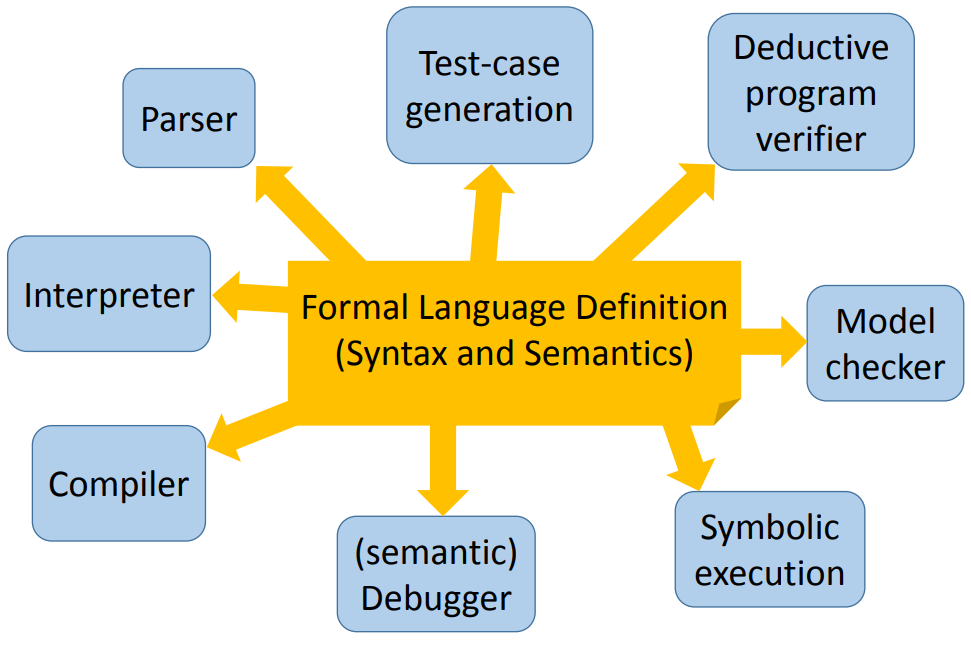
\includegraphics[width=1.0\linewidth]{img/kidea.png}
\end{frame}

% V K již byla popsána sémantika Pythonu, JavaScriptu, C a dalších jazyků.
% Nad sémantikou jazyka C byl postaven komerční nástroj pro detekci
% nedefinovaného chování RV-Match a tato sémantika je poslední
% dva roky rozšiřována o podporu jazyka C++, které je zatím jen v experimentální fázi.
\begin{frame}{C/C++ @ K}
\begin{itemize}
\item Již formalizováno: Python, JavaScript, C
\pause \item využití C: RV-Match \\

\includegraphics[width=0.3\linewidth]{img/rvmatch.png}
\pause \item experimentálně: C rozšiřováno o podporu C++
\end{itemize}
\end{frame}

% Zadání, cíle, konkrétní věci, nalezené chyby apod.
\section{Cíle práce}


% Cílem mé práce bylo rozšířit stávající prototyp
% C++ sémantiky v K o dosud neimplementované vlastnosti tohoto jazyka.

% První vlastností, kterou jsem zamýšlel implementovat,
% jsou výčtové typy. V projektu sice výčtové typy byly implementovány,
% ale jen pro jazyk C. V jazyce C++ se výčtové typy chovají trošku jinak,
% navíc ve standardu C++11 (z roku 2011) přibyla nová varianta těchto typů.

% Další vlastností, kterou jsem chtěl implementovat, byla podpora vykonávání kódu
% v době překladu. Od standardu C++11 je možné označit některou z funkcí
% jako 'constexpr', což v praxi znamená, že volání takovéto funkce je možné
% vyhodnotit již v době překladu. Výpočet pak není nutné dělat za běhu,
% což může výrazně pomoci jak výkonu programu, tak čitelnosti jeho kódu.
% Výsledek výpočtu je navíc možné použít i na místech, kde jazyk vyžaduje použití konstanty.
% A ano - jazyk C++ je díky této vlastnosti turingovsky úplný už v době překladu.
% Jenže on byl turingovsky úplný již dávno předtím.

% Přestože jsem to původně neměl v úmyslu, na popud jednoho z hlavních vývojářů projektu
% jsem implementoval vlastnost, která se nazývá "nulová inializace tříd".
% Myslel jsem si, že to bude hračka, ale zabralo mi to dost dlouhou dobu.
% Jedním z důvodů byla i chyba v projektu, která se projevovala až tehdy,
% když jsem se pokoušel nulovou inicializaci naimplementovat. Chybou byl
% nedeterminismus v sémantice, který umožňoval interpretovat některé programy vícero způsoby.

% Tím se dostáváme k poslednímu bodu - opravě některých stávajících chyb.
% Projekt C++ sémantiky v K je stále v experimentální fázi,
% a tak se při práci častokrát stalo, že jsem narážil
% na nějakou chybu či nedokončenou implementaci. Opravoval jsem zejména
% ty, které mi nějak překážely.

% Ještě doplním, že z těchto čtyř bodů byly jen první dva
% součástí mého oficiální zadání.

% čas: 2min 15s
%\begin{frame}{Cíle práce}
%\begin{itemize}
%\pause \item výčtové typy (\texttt{enum})
%\pause \item vykonávání kódu v době překladu (\texttt{constexpr})
%\pause \item nulová inicializace tříd
%\pause \item oprava stávajících chyb v projektu
%\end{itemize}
%\end{frame}

\begin{frame}[fragile]{Výčtové typy (\texttt{enum})}
\begin{lstlisting}[language=C++]
enum E0 { A = 5, B = A + 3 };
enum E1 : char;
enum class E2 : unsigned int;
enum class E3;
enum E5 { A, B } __attribute__((packed));
std::underlying_type_t<E5> x = 5;
\end{lstlisting}
\end{frame}

\begin{frame}[fragile]{Vykonávání kódu v době překladu (\texttt{constexpr})}
\begin{lstlisting}
constexpr int fact(int n) {
	return n <= 1 ? 1 : n * fact(n - 1);
}
int main() {
	constexpr int f_4 = fact(4);
	enum class Facts {
		F_4 = f_4,
		F_5 = fact(5)
	};
	assert(int(Facts::F_4) == 24);
	assert(int(Facts::F_5) == 120);
}
\end{lstlisting}
\end{frame}

\begin{frame}[fragile]{Nulová inicializace tříd}
\begin{lstlisting}
struct S {
	virtual ~S() = default;
	int x;
};

S s1;
S s2{};
assert(s1.x == 0); // ok
assert(s2.x == 0); // fail
\end{lstlisting}
\end{frame}

\begin{frame}{Oprava stávajících chyb v projektu}
\includegraphics[width=0.5\linewidth]{img/bug.jpg}
\end{frame}

% Zde budou nějaké děsivé příklady
%\subsection{Intriky}


% Co se povedlo, co jsem se naucil, jake jsou moje dalsi plany.

% Možná mohu říci, že práce s K frameworkem sice byla složitá v tom smyslu,
% že jsem se musel naučit hodně nových věcí, vžít se do nového programovacího paradigmatu
% apod, ale nebyla potřeba žádná hluboká matematická znalost (žádné fixpointy apod).
\section{Výsledky \& co dál?}

\begin{frame}{Výsledky}
\begin{itemize}
\pause \item \texttt{enum} - vše hotovo, většina je v upstream
\pause \item \texttt{constexpr} - elegantní proof of concept
\pause \item nulová inicializace - hotovo
\pause \item opravy chyb - některé přijaty do upstreamu
\pause \item nalezené chyby v GCC, Clang, standardu C++
\end{itemize}
\end{frame}

\begin{frame}{Co dál?}
\begin{itemize}
\pause \item Vše hotové do upstreamu.
\pause \item Dokončit \texttt{constexpr}.
\pause \item Šablony, vlákna, bitová pole, fold expressions, \ldots
\pause \item Jak řešit vývoj jazyka?
\pause \item Spolupráce s RuntimeVerification inc.
\pause \item Kontrakty.
\end{itemize}
\end{frame}


\begin{frame}[fragile=singleslide]{Ochutnávka}
\begin{lstlisting}
template <typename It>
bool is_sorted(It begin, It end);

/*
 * \pre valid_range(begin, end);
 * \post is_sorted(begin, end);
 */
template <typename It>
void sort(It begin, It end);
\end{lstlisting}
\end{frame}


\begin{frame}{Kontrakty}
\begin{itemize}
\pause \item Jak jim dát sémantiku?
\pause \item Volání běžných funkcí v pre/postcondition.
\pause \item A co když mají efekty? A co když ty jsou ohraničené?
\pause \item Jak je verifikovat?
\pause \item Jak využít existující abstrakce? A vzory?
\end{itemize}
\end{frame}


\begin{frame}{Zdroje}
\begin{itemize}
\item Mapa C++ \url{https://fearlesscoder.blogspot.cz/2017/02/the-c17-lands.html}
K diagram \url{http://fsl.cs.illinois.edu/index.php/From\_Rewriting\_Logic,\_to\_Programming\_Language\_Semantics,\_to\_Program\_Verification} \\
\item RV-Match logo \url{https://runtimeverification.com/match/}
\item Brouk \url{http://cliparting.com/free-bug-clipart-30526/}
\end{itemize}
\end{frame}

\backupbegin

\section{Bonusy}


% Tohle bych mohl mozna presunout do bonusu.
% Tady bych jenom dodal, že nalezení chyb v překladačíh
% nebo standardech programovacích jazyků není až tak moc neobvyklé,
% zvlášť v kontextu formalizace těchto jazyků - JavaScript, Ethereum.
%\subsection{Chyby nalezené v jiných projektech}

% Během práce jsem hodně pracoval se standardem jazyka C++,
% a když jsem o C++ zjišťoval nové věci, prakticky jsem je zkoušel
% na malých příkladech. Kladl jsem si otázku, "co se stane, když..."?
% Tímto způsobem jsem našel chybu v překladači GCC.
% Kód na slajdu je platný C++ kód, a Clang nebo MSVC jej bez problémů zkompilují,
% nicméně GCC jej odmítne zparsovat. Chybu jsem nahlásil do bugzilly projektu
% a jeden z hlavních vývojářů ji potvrdil.
\begin{frame}[fragile=singleslide]{GCC bug}
\begin{lstlisting}
enum E : int;
enum ::E : int{};
\end{lstlisting}
\end{frame}

% Další chybu jsem objevil v překladači clang.
% Chyba se týká toho, v jakém scope žijí konstanty výčtového typu
% (v našem případě konstanty A a B).
%
% Podle jednoho z vývojářů překladače clang, konkrétně správce
% C++ frontendu tohoto překladače, se příčina této chyby projevuje
% i v jiných případech, ve kterých nemá vliv na korektnost, ale jen
% na výkon překladače.
\begin{frame}[fragile=singleslide]{Clang bug}
\begin{lstlisting}
namespace N { enum E : int; }
enum N::E : int {A,B};
namespace N {
    int x = int(::N::B); // 1
}
int y = int(::A); // 2
int z = int(A); // 3
\end{lstlisting}
\end{frame}

\begin{frame}[fragile=singleslide]{C++ standard bug}
\begin{lstlisting}
enum class E {
    A,
    B = E::A // 1
};
\end{lstlisting}
Jaký typ má \lstinline|E::A| v (1)?
\end{frame}

% Btw v C++ sémantice stále ještě není implementován switch.
% Po otázkách - kdyby chtěli vědět něco dalšího, rád si s nima popovídám.
% Co jsem se naučil: komunikace na dálku je fuška.
% S lidma z RV a UIUC se mi spolupracovalo dobře.

\backupend

\end{document}